\documentclass[12pt,a4paper]{scrartcl}
\usepackage[utf8]{inputenc}
\usepackage{amsmath, amssymb}
\usepackage{array}
\usepackage{listings} 
\usepackage{epsfig} 
\usepackage{graphicx} 
\usepackage{rotating} 
\usepackage{lscape}
\usepackage{color}
\usepackage{xcolor} 
\usepackage{subfig}
\usepackage{everysel}
\usepackage{natbib}
\usepackage{times}

% page size
\setlength{\parskip}{0.4\baselineskip}
\setlength{\textheight}{21 cm}
\setlength{\textwidth}{15 cm}
\setlength{\topmargin}{0.5 cm}
\setlength{\hoffset}{-0,5 cm}
\setlength{\voffset}{-0,5 cm}
\setlength{\headsep}{1 cm}
\setlength{\oddsidemargin}{1 cm}
\setlength{\evensidemargin}{1 cm}
\marginparwidth 1.8cm \marginparsep 10pt
\setlength{\belowcaptionskip}{5pt}
\setlength{\belowcaptionskip}{5pt}

% caption style
\renewcommand{\captionfont}{\footnotesize}
\renewcommand{\captionlabelfont}{\bf \sffamily}
\setcapindent{0pt}

% table rulers
\newcommand{\toprule}{\hline\hline}
\newcommand{\midrule}{\hline}
\newcommand{\botrule}{\hline\hline}

% differential opterators
\newcommand{\dd}[2]{\frac{\partial #1}{\partial #2}}
\newcommand{\ddd}[3]{\frac{\partial^2 #1}{\partial #2 \partial #3}}
\newcommand{\DD}[2]{\frac{\mathrm{d} #1}{\mathrm{d} #2}}
\newcommand{\DDsquare}[2]{\frac{\mathrm{d}^2 #1}{\mathrm{d} #2^2}}
\newcommand{\DDD}[3]{\frac{\mathrm{d}^2 #1}{\mathrm{d} #2\mathrm{d} #3}}


% hyperlink color
\usepackage[colorlinks=true, linkcolor=black, citecolor=black, filecolor=black, 
urlcolor=black]{hyperref}
%\usepackage[colorlinks=true, linkcolor=blue, citecolor=blue, filecolor=blue, urlcolor=blue]{hyperref}

% comments
\newcommand{\ar}[1]{{\color{red}#1}}

\begin{document}

\section*{SUPPLEMENTARY INFORMATION}
\section*{Data2Dynamics: a modeling environment tailored to parameter 
estimation in dynamical systems}

\noindent A.~Raue\,$^{1,}$, B.~Steiert$^{2}$, M.~Schelker$^{3}$, C.~Kreutz$^{2}$, H.~Hass$^{2}$, J.~Vanlier$^{2}$, C.~T\"onsing$^{2}$, L.~Adlung$^{4}$, R.~Engesser$^{2}$, W.~Mader$^{2}$, T.~Heinemann$^{5}$, J.~Hasenauer$^{6}$, M.~Schilling$^{4}$, T.~H\"ofer$^{5}$, E.~Klipp$^{2}$, B.~Sch\"oberl$^{1}$, F.~Theis$^{6}$, U.~Klingm\"uller$^{4}$ and J.~Timmer\,$^{2,7,8}$

\noindent $^{1}$Merrimack Pharmaceuticals Inc., 02139 Cambridge, MA, USA\\
$^{2}$University of Freiburg, Institute for Physics, 79104 Freiburg, Germany\\
$^{3}$Humboldt-Universit\"at zu Berlin, Theoretical Biophysics, 10115 Berlin, Germany\\
$^{4}$German Cancer Research Center, 69120 Heidelberg, Germany.\\
$^{5}$BioQuant, University of Heidelberg, 69120 Freiburg, Germany\\
$^{6}$Helmholtz Center Munich, 85764 Neuherberg, Germany.\\
$^{7}$BIOSS, University of Freiburg, 79104 Freiburg, Germany\\
$^{8}$Zentrum f\"ur Biosystemanalyse, University of Freiburg, 79104 Freiburg, 
Germany

\subsection*{Implementation and System Requirements} 
The Data2Dynamics modeling environment is MATLAB-based, open source and freely available. 
MATLAB R2012 or later recommended, MATLAB Optimization Toolbox and Symbolic Math Toolbox required. 
Windows, Mac and Linux systems are supported. For MATLAB mex compilation under Windows systems, freely available Windows SDK 7.1 is required.

\subsection*{Availability, Documentation and Bug Reports}
The Data2Dynamics modeling environment is available at \href{http://www.data2dynamics.org}{{\bf http://www.data2dynamics.org}}. 
The website contains full documentation and a description of the example applications. Code changes between version can be tracked, 
bug reports can be issued and code improvement and additional functionality can be submitted. Participation is highly welcome! 

\subsection*{Contact}
\href{andreas.raue@fdm.uni-freiburg.de}{andreas.raue@fdm.uni-freiburg.de} \\
\href{jeti@fdm.uni-freiburg.de}{jeti@fdm.uni-freiburg.de}

% table of contents
\renewcommand*\contentsname{Contents}
\tableofcontents

\section{Efficient solution of the ODE system} \label{sec:ode_solvers}

The dynamics of biochemical reaction networks, i.e.~the time evolution of the concentrations 
of the involved molecular compounds, can be modeled by a system of ordinary 
differential equations (ODE)
\begin{equation}
	\DD{}{t}{\mathbf{x}}(t, \boldsymbol{\theta}) = \mathbf{f}_{x}(\mathbf{x}(t, 
\boldsymbol{\theta}), \mathbf{u}(t, \boldsymbol{\theta}), \boldsymbol{\theta}). 
\label{odesystem2}
\end{equation}
The variables $\mathbf{x}$ correspond to the dynamics of the concentration of $n$ 
molecular compounds such as hormones, proteins in different phosphorylation states, 
mRNA or complexes thereof. A time-dependent experimental treatment that alters the 
dynamical behavior of the system can be incorporated by the function $\mathbf{u}(t, 
\boldsymbol{\theta})$. To be able to handle unknown quantities in these driving inputs, we 
consider the case where the function $\mathbf{u}$ can also be parameter dependent. For 
instance, $\mathbf{u}$ can represented by a smoothing spline as described in 
\citet{Schelker:2012uq}. The initial state of the system is described by 
\begin{equation}
	\mathbf{x}(0, \boldsymbol{\theta}) = \mathbf{f}_{x_0}(\boldsymbol{\theta}). 
\label{init_ode_sys}
\end{equation}	
The set of parameters $\boldsymbol{\theta} = \{\theta_1 \dots \theta_l\}$ determines the  
dynamics. Except for very small systems the analytical solution to Equation~(\ref{odesystem2}) is 
not available any more. Therefore, the dynamics have to be computed by a numerical ODE 
solver. For ODE systems describing biochemical reactions, a reaction flux occurs multiple times in the right 
hand side of Equation~(\ref{odesystem2}). Therefore, the right hand side of 
Equation~(\ref{odesystem2}) can usually be decomposed into a stoichiometry matrix $
\mathbf{N}$ and rate equations $\mathbf{v}$ of the reaction fluxes of the molecular 
interactions
\begin{equation}
	\mathbf{f}_{x}(\mathbf{x}(t, \boldsymbol{\theta}), \mathbf{u}(t, \boldsymbol{\theta}), 
\boldsymbol{\theta}) = \mathbf{N} \cdot \mathbf{v}(\mathbf{x}(t, \boldsymbol{\theta}), 
\mathbf{u}(t, \boldsymbol{\theta}), \boldsymbol{\theta}). \label{fluxsystem2}
\end{equation}
The stoichiometry matrix $\mathbf{N}$ is sparse. For numerical efficiency it is 
advantageous to precompute the reaction fluxes $\mathbf{v}$ and use 
Equation~(\ref{fluxsystem2}) as right hand side of the ODE system. 

The timescales of cellular processes can differ by orders of magnitude. As a 
consequence, the resulting nonlinear ordinary differential equations can be stiff, for a 
general introduction into this topic see \citet{Lambert:1977fk}. Roughly speaking, stiffness 
is characterized by the presence of at least one rapidly damped mode whose time 
constant is small compared to the timescale of the remaining dynamics. In the presented 
software package, the CVODES solver \citep{Hindmarsh:2005fb} that is implemented in C for 
efficiency is used. It solves both stiff and non-stiff systems. The methods used in CVODES 
are variable-order, variable-step multistep methods, based on the Adams-Moulton 
formulas for non-stiff and on the Backward Differentiation Formulas for stiff systems 
\citep{Byrne:1975uq}. CVODES also allows for efficient simultaneous solution of the 
sensitivity equations, see Section~\ref{sec:ode_simu}. For convenience the solver was 
implemented in combination with a MATLAB mex-interface. For numerical efficiency it is 
favorable to provide the Jacobian matrix $\mathbf{J}$ of the right hand side of 
Equation~(\ref{odesystem2}) with respect to the dynamic variables $\mathbf{x}$ 
\begin{equation}
	\mathbf{J} = \dd{\mathbf{f}_{x}}{\mathbf{x}} = \mathbf{N} \cdot \dd{\mathbf{v}}
{\mathbf{x}}\label{jac_mat}
\end{equation}
to the ODE solver. Here, again, Equation~(\ref{fluxsystem2}) can be exploited to simplify 
computations.

\section{Parallelization of computations} \label{sec:parallel}

Experimental measurements are mathematically represented by functional mappings
\begin{equation}
    {\bf y}(t,{\boldsymbol \theta}) = {\bf f}_y({\bf x}(t,{\boldsymbol \theta}),{\bf u}(t,{\boldsymbol 
\theta}),{\boldsymbol \theta}). \label{eq:obs}
\end{equation}
For each experimental condition Equation~(\ref{fluxsystem2}) and~(\ref{jac_mat}) have to 
be modified according to the treatment applied. This can for example be a different 
network structure represented by $\mathbf{N}$ due to knock-out, knock-in, or inhibition 
experiments or different experimental treatments incorporated by the function $\mathbf{u}
(t, \boldsymbol{\theta})$ or $\mathbf{f}_{x_0}(\boldsymbol{\theta})$ . Consequently, there 
can be as many variants of the ODE systems as experimental conditions, each having an 
individual numerical solution for the dynamics. For comparing the whole model to 
the experimental data, given a specific set of candidate parameters, all ODE variants have 
to be solved. During parameter estimation many evaluations of the whole model are 
necessary. This can be a numerically intensive task. All ODE variants can be solved 
independently, therefore this problem is ideal for parallel computing. Here, a multithreading 
technique was employed that results in a significant acceleration on multi-core machines. 
For the model of \citet{Bachmann:2011fk}, 24 ODE variants have to be solved consecutively. 
As displayed in Figure~\ref{Acceleration}, the speed up increases as expected with 
increasing number of threads used.

\begin{figure}
\begin{center}
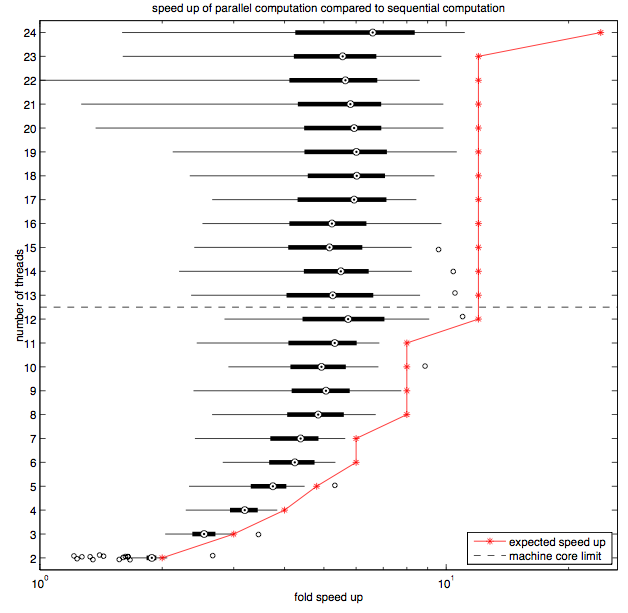
\includegraphics[width=\textwidth]{./figures_QDM/bachmann_MSB2011_speed_up_test.png}
\end{center}
\caption{Acceleration of numerical computations for the solution of ODE systems by 
multithreading. For each bar, 24 variants of the ODE systems used for the model by 
\citet{Bachmann:2011fk} were solved for 1000 randomly drawn sets of parameters 
using a Latin hypercube sampling strategy. The red line displays the theoretically possible
acceleration. A 12-core processor was used in this benchmark.}
\label{Acceleration}
\end{figure}

\section{Maximum Likelihood estimation and deterministic optimization 
algorithms} \label{sec:det_optimization}
Numerical optimization algorithms try to find the argument $\boldsymbol{\hat \theta}$ that 
minimizes the value of an objective function $L(\boldsymbol{\theta})$. In the case of 
independently and normally distributed measurement noise the objective function for 
maximum likelihood estimation is given by
\begin{equation}
	L(\boldsymbol{\theta}) = \sum_{k=1}^m \sum_{i=1}^{d_k}\, 2\log(\sqrt{2 \pi}) + 
2\log(\sigma_k(t_i, \boldsymbol{\theta}))\, + \left(\frac{y_{ki}^\dagger - y_{k}(t_{i}, 
\boldsymbol{\theta})}{\sigma_k(t_i, \boldsymbol{\theta})}\right)^2 \label{llhoodfun2}
\end{equation}
where $L(\boldsymbol{\theta}) =  - 2\cdot \log(\mathcal{L}(\mathbf{y}^\dagger|\,
\boldsymbol{\theta}))$ of the likelihood $\mathcal{L}$, ${\bf y}^\dagger$ is the experimental 
data and normally distributed measurement noise is assumed. The variance can be a 
parameterized function $\sigma_k(t_i, \boldsymbol{\theta})^2$, and the corresponding 
parameter can be estimated together with the other parameters. In the following we will 
refer to both $\mathcal{L}$ and $L$ simply as likelihood. The minimum of 
$L(\boldsymbol{\theta})$ is called the best fit of the model to the experimental data and the 
corresponding parameters $\boldsymbol{\hat \theta}$ are the maximum likelihood 
estimates since they maximize $\mathcal{L}$. Numerical algorithms have to be used to 
estimate the parameters because of the non-linearity of the optimization problem. 
Deterministic optimization algorithms try to take steps of $\Delta \boldsymbol{\theta}$ that 
successively decrease the value of $L(\boldsymbol{\theta})$ beginning from an initial 
guess $\boldsymbol{\theta}_0$ \citep{Press:1990rw}. The parameters are updated by $
\boldsymbol{\theta}_{i+1} = \boldsymbol{\theta}_{i} + \Delta \boldsymbol{\theta}$. To 
generate steps, deterministic optimization algorithms evaluate derivatives of the likelihood. 
The Data2Dynamics software also implements stochastic optimization algorithms, such as
 particle swarm optimization, differential evolution, simulated annealing, genetic algorithm 
 and others, see \citet{Kronfeld:2010fk} for a detailed description of methods an 
 implementation, for a benchmark comparison, see \citet{Raue:2012zt}. The most efficient 
 and reliable algorithm for parameter estimation in our hands is a deterministic trust region 
 approach combined with multi-start strategy to map out local minima. Parameters can and 
 should be estimated on a logarithmic scale.

\paragraph{Gradient descent method.}
The \emph{gradient descent} method takes steps 
\begin{equation}
	\Delta \boldsymbol{\theta} = - \gamma \cdot \nabla L(\boldsymbol{\theta}) 
\label{gradientstep}
\end{equation}	
down the gradient of $L$. $\gamma$ is chosen sufficiently small such that a decrease in 
the objective function $L(\boldsymbol{\theta}_{i+1}) < L(\boldsymbol{\theta}_{i})$ can be 
guaranteed. It is well known that this simple method exhibits only linear convergence rate 
\citep{Stoer:2005fk}. Furthermore, for non-linear problems the method has convergence 
problems if the objective function contains long and flat valleys \citep{Rosenbrock:1960fk}. 
These structures are typical for likelihood functions of ODE models describing biochemical 
reaction networks, sometimes referred to as \emph{sloppiness} \citep{Gutenkunst:2007ct}. 

\paragraph{Newton and quasi-Newton methods.}
To circumvent convergence problems of the gradient descent method, the \emph{Newton} 
method applies a second order Taylor expansion of the objective function
\begin{equation}
	\tilde L(\Delta \boldsymbol{\theta}) = L(\boldsymbol{\theta}) + \mathbf{g} \cdot \Delta 
\boldsymbol{\theta} + \frac{1}{2} \Delta \boldsymbol{\theta}^\top \cdot \mathbf{H} \cdot 
\Delta \boldsymbol{\theta}, \label{2taylor}
\end{equation}
where $\mathbf{g} = \nabla L(\boldsymbol{\theta})$ is the gradient and $\mathbf{H} = 
\nabla^\top\nabla\, L(\boldsymbol{\theta})$ is the Hessian matrix of $L(\boldsymbol{\theta})
$. For the calculation of $\mathbf{g}$ and $\mathbf{H}$ for ODE models, see in the 
Section~\ref{sec:derivativies}. The Newton step is given by 
\begin{equation}
	\Delta \boldsymbol{\theta} = -\mathbf{H}^{-1} \cdot \mathbf{g} \label{newtonstep}
\end{equation}
and leads, if the approximation is good, to the optimal solution in a single step. 
Compared to the gradient descent method, the Newton method exhibits quadratic 
convergence rate \citep{Stoer:2005fk}. The performance decreases considerably as the 
goodness of the approximation decreases. In this case and also for non-positive definite $
\mathbf{H}$, the method can become unstable, i.e.~decrease in the objective function is 
not guaranteed for each step. 

Instead of computing $\mathbf{H}$ directly from the model, \emph{quasi-Newton} methods 
build up information about $\mathbf{H}$ iteratively from sequential evaluations of $
\mathbf{g}$, see for example the \emph{Broyden-Fletcher-Goldfarb-Shanno} update 
\citep{Shanno:1970fk}. Iterative approaches are especially useful if computation of second order
derivatives is not feasible. As explained in Section~\ref{sec:derivativies}, this is not 
necessary for ODE models.

\paragraph{Levenberg-Marquardt method.}
To circumvent stability problems of Newton methods the \emph{Levenberg-Marquardt} 
method \citep{Marquardt:1963uq} uses 
\begin{equation}
	\Delta \boldsymbol{\theta} = -(\mathbf{H} + \lambda \cdot \mathbf{1})^{-1} \cdot 	
\mathbf{g}. 
\end{equation}	
For $\lambda \rightarrow 0$ the Newton step of Equation~(\ref{newtonstep}) is obtained, 
for $\lambda \rightarrow \infty$ the gradient descent step direction of 
Equation~(\ref{gradientstep}) is obtained. With increasing $\lambda$, the step size is 
reduced. Consequently, $L(\boldsymbol{\theta}_{i+1}) < L(\boldsymbol{\theta}_{i})$ can be 
guaranteed but also efficient Newton steps can be performed if the approximation is a 
good one. It can be shown that the quality of the approximation~(\ref{2taylor}) increases in 
the proximity of an optimum in the likelihood \citep{Seber:2003kq}.

\paragraph{Trust region methods.}
Closely related to the Levenberg-Marquardt method are \emph{trust region} methods 
\citep{Coleman:1996fk}. These methods minimize Equation~(\ref{2taylor}) under the 
constraint $\left|\left| \Delta \boldsymbol{\theta} \right|\right| \leq \mu $ to generate the trial 
step. The parameter $\mu$ that defines the radius of the trust region has a similar effect 
as $\lambda$ in the Levenberg-Marquardt method, i.e.~for small enough $\mu$, 
$L(\boldsymbol{\theta}_{i+1}) < L(\boldsymbol{\theta}_{i})$ can be guaranteed.

Here, the trust region algorithm LSQNONLIN implemented in MATLAB is used. To reduce expensiveness of the constrained minimization of 
Equation~(\ref{2taylor}), the LSQNONLIN algorithm formulates a two-dimensional 
approximation to Equation~(\ref{2taylor}) by a plane in parameter space. The gradient 
descent direction of Equation~(\ref{gradientstep}) and an approximate Newton step of 
Equation~(\ref{newtonstep}) span the plane of this new approximation. Since the gradient 
decent direction is contained $L(\boldsymbol{\theta}_{i+1}) < L(\boldsymbol{\theta}_{i})$ 
for small $\mu$ can be guaranteed again. The approximate Newton step is obtained by 
\emph{preconditioned conjugated gradients} methods \citep{Barrett:1994uq} instead of 
using direct matrix inversion that is considerably slower for large parameter space.

\section{Derivative calculations for ODE models} \label{sec:derivativies}
For deterministic optimization algorithms, the gradient $\mathbf{g} = \nabla 
L(\boldsymbol{\theta})$ and Hessian matrix $\mathbf{H} = \nabla^\top\nabla\, 
L(\boldsymbol{\theta})$ of the likelihood are required. The first term in 
Equation~(\ref{llhoodfun2}) is a constant. The last term is the well-known weighted sum of 
squared residuals, sometimes denoted by $\chi^2(\boldsymbol{\theta})$. 
Equation~(\ref{llhoodfun2}) can be reformulated
\begin{eqnarray}
	L(\boldsymbol{\theta}) & = & const + \sum_{k=1}^m \sum_{i=1}^{d_k}\, 
2\log(\sigma_k(t_i, \boldsymbol{\theta}))\, +  \left(\frac{y_{ki}^\dagger - y_{k}(t_{i}, 
\boldsymbol{\theta})}{\sigma_k(t_i, \boldsymbol{\theta})}\right)^2 \label{llhoodfun3ij} \\
	& = & const + \sum_{q=1}^{s} \tilde r_{q}(\boldsymbol{\theta})^2 + \sum_{q=1}^{s}  
r_{q}(\boldsymbol{\theta})^2 \label{llhoodfun3}
\end{eqnarray}
where the new sum index $q$ runs over all $i$ and $j$ in ($\ref{llhoodfun3ij}$) and $s = 
\sum_{k=1}^m d_k$. The first sum contains the elements 
\begin{equation}
	\tilde r_{q}(\boldsymbol{\theta}) = \sqrt{2\log(\sigma_k(t_i, \boldsymbol{\theta}))}. 
\label{rl1}
\end{equation}	
Since $\log(\sigma_k(t_i, \boldsymbol{\theta}))$ can be negative, in practice 
\begin{equation}
	\tilde r_{q}(\boldsymbol{\theta}) = \sqrt{2\log(\sigma_k(t_i, \boldsymbol{\theta})) + c} 
\label{rl2}
\end{equation}
is used, where $c$ is a large enough constant. The constant $c$ adds another constant to 
Equation~(\ref{llhoodfun3}) but does not change the shape of the likelihood function, 
hence, maximum likelihood estimation and confidence intervals are not affected. The second sum contains the 
normalized residuals 
\begin{equation}
	r_{q}(\boldsymbol{\theta}) = \frac{y_{ki}^\dagger - y_{k}(t_{i}, \boldsymbol{\theta})}
{\sigma_k(t_i, \boldsymbol{\theta})}.  \label{rl3}
\end{equation}
The gradient can then be obtained by
\begin{equation}
	\mathbf{g} = \DD{L}{\boldsymbol{\theta}} = 2 \sum_{q=1}^{s} \left( {\tilde r}_{q} \cdot 
\DD{{\tilde r}_{q}}{\boldsymbol{\theta}} + {r}_{q} \cdot \DD{{r}_{q}}{\boldsymbol{\theta}} 
\right)
\end{equation}
and the Hessian matrix by 
\begin{equation}
	\mathbf{H} = \DDsquare{L}{\boldsymbol{\theta}} = 2 \sum_{q=1}^{s} \left( \DD{{\tilde r}
_{q}}{\boldsymbol{\theta}} \cdot \DD{{\tilde r}_{q}}{\boldsymbol{\theta}} + {\tilde r}_{q} \cdot 
\DDsquare{{\tilde r}_{q}}{\boldsymbol{\theta}} + \DD{{r}_{q}}{\boldsymbol{\theta}} \cdot 
\DD{{r}_{q}}{\boldsymbol{\theta}} + {r}_{q} \cdot \DDsquare{{r}_{q}}{\boldsymbol{\theta}} 
\right). \label{fullH}
\end{equation}
For the following calculations we look at each component $q$ individually and drop the 
index for better readability. First and second order derivatives of ${\tilde r}$ can be 
evaluated by
\begin{equation}
	\DD{{\tilde r}}{\boldsymbol{\theta}}  = \frac{1}{{\tilde r}{\sigma}} \DD{{\sigma}}
{\boldsymbol{\theta}} \label{reserrfirst}
\end{equation}
and
\begin{equation}
	\DDsquare{{\tilde r}}{\boldsymbol{\theta}}  = \frac{1}{{\tilde r} {\sigma}}
\frac{\mathrm{d}^2{\sigma}}{\mathrm{d} \boldsymbol{\theta}^2} - \frac{1}{{\tilde r} {\sigma}^2}\DD{{\sigma}}
{\boldsymbol{\theta}}\cdot \DD{{\sigma}}{\boldsymbol{\theta}} - \frac{1}{{\tilde r}^2 {\sigma}}
\DD{{\sigma}}{\boldsymbol{\theta}}\cdot \DD{{\tilde r}}{\boldsymbol{\theta}}.
\end{equation}
First order derivatives of ${r}$ can be calculated by
\begin{equation}
	\DD{{r}}{\boldsymbol{\theta}}  = \frac{-1}{{\sigma}} \DD{{y}}{\boldsymbol{\theta}} - 
\frac{{r}}{{\sigma}} \DD{{\sigma}}{\boldsymbol{\theta}.} \label{resderivatives}
\end{equation}
Let ${f}_\sigma$ be the equation for the variance $\sigma_k(t_i, \boldsymbol{\theta})^2$. 
We can then further obtain
\begin{equation}
\DD{{\sigma}}{\boldsymbol{\theta}} = \dd{f_\sigma}{{y}}\DD{{y}}{\boldsymbol{\theta}} + 
\dd{f_\sigma}{\boldsymbol{\theta}} \label{sigmaderivatives}
\end{equation} 
and
\begin{equation}
 \DDsquare{{\sigma}}{\boldsymbol{\theta}} = 2\ddd{f_\sigma}{y}{\boldsymbol{\theta}} 
\DD{{y}}{\boldsymbol{\theta}} + \dd{f_\sigma}{y}{\color{red}\DDsquare{{y}}
{\boldsymbol{\theta}}} + \frac{\partial^2f_\sigma}{\partial y^2}\DD{{y}}{\boldsymbol{\theta}}
\DD{{y}}{\boldsymbol{\theta}} + \DDsquare{f_\sigma}{\boldsymbol{\theta}}. \label{ddsigma}
\end{equation}
With the equation for the measurements ${f}_y$ we can resolve
\begin{equation}
	\DD{{y}}{\boldsymbol{\theta}} = \dd{{f}_y}{\mathbf{x}} {\color{red}\DD{\mathbf{x}}
{\boldsymbol{\theta}}} + \dd{{f}_y}{\mathbf{u}} \DD{\mathbf{u}}{\boldsymbol{\theta}} + 
\dd{{f}_y}{\boldsymbol{\theta}}. \label{sderive}
\end{equation}
All expressions in Equations~(\ref{reserrfirst}-\ref{sderive}) can be calculated analytically 
except for terms indicated in red. In Equation~(\ref{sderive}), the derivatives of the 
dynamic variables $\mathrm{d} \mathbf{x}/\mathrm{d} \boldsymbol{\theta}$, the so called \emph{sensitivities}, 
can be calculated numerically, as described in Section~\ref{sec:ode_simu}. The calculation 
of $\mathrm{d}^2 {y}/\mathrm{d} \boldsymbol{\theta}^2$  involves second order sensitivities $\mathrm{d}^2 \mathbf{x}/\mathrm{d} 
\boldsymbol{\theta}^2$ of the dynamics that are expensive to evaluate numerically. 

The calculation of the last term in Equation~(\ref{fullH}), ${r} \cdot \mathrm{d}^2{r}/\mathrm{d}
\boldsymbol{\theta}^2$ is more complicated. Following the argumentation in~\citet[Section 
15.5 Nonlinear Models]{Press:1990rw}, in the proximity of a good model fit, the normalized 
residuals ${r}$ fluctuate in an uncorrelated manner around zero. Therefore, the term tends to cancel out 
when summed over $q$ and quadratic convergence of optimization algorithms using 
Newton steps can be obtained without calculating second order sensitivities. 

However, if measurement noise parameters are estimated as well, the argumentation is 
more involved. In the following, the parameters are collected in three groups: $
\boldsymbol{\theta}_y$ are parameters that only affect the observables ${y}$, $
\boldsymbol{\theta}_s$ are parameters that only affect the measurement noise ${\sigma}$ 
and $\boldsymbol{\theta}_{b}$ are parameters that affect both. Correspondingly, the last 
term in Equation~(\ref{fullH}) can be reformulated to
\begin{displaymath}
{r} \cdot \DDsquare{{r}}{\boldsymbol{\theta}} = {r} \cdot \left( 
\begin{array}{ccc}
\DDsquare{{r}}{\boldsymbol{\theta}_y} & \DDD{{r}}{\boldsymbol{\theta}_y}
{\boldsymbol{\theta}_s} & \DDD{{r}}{\boldsymbol{\theta}_y}{\boldsymbol{\theta}_b} \\
\\
\DDD{{r}}{\boldsymbol{\theta}_s}{\boldsymbol{\theta}_y} & \DDsquare{{r}}
{\boldsymbol{\theta}_s} & \DDD{{r}}{\boldsymbol{\theta}_s}{\boldsymbol{\theta}_b} \\
\\
\DDD{{r}}{\boldsymbol{\theta}_b}{\boldsymbol{\theta}_y} & \DDD{{r}}{\boldsymbol{\theta}
_b}{\boldsymbol{\theta}_s} & \DDsquare{{r}}{\boldsymbol{\theta}_b}
\end{array} 
\right).
\end{displaymath}
With Equation~(\ref{rl3}) we can calculate
\begin{eqnarray}
	{r} \cdot \DDsquare{{r}}{\boldsymbol{\theta}_y} & = & \frac{-{r}}{{\sigma}}{\color{red}
\DDsquare{{y}}{\boldsymbol{\theta}_y}} \label{problem1}
	\\
	{r} \cdot \DDsquare{{r}}{\boldsymbol{\theta}_s} & = & \frac{{r}^2}{{\sigma}
^2}\DD{{\sigma}}{\boldsymbol{\theta}_s}\DD{{\sigma}}{\boldsymbol{\theta}_s} - \frac{{r}^2}
{{\sigma}}\DDsquare{{\sigma}}{\boldsymbol{\theta}_s} 
	\\
	{r} \cdot \DDsquare{{r}}{\boldsymbol{\theta}_b} & = & \frac{{r}}{{\sigma}^2}\DD{{y}}
{\boldsymbol{\theta}_b}\DD{{\sigma}}{\boldsymbol{\theta}_b} - \frac{{r}}{{\sigma}}\DD{{r}}
{\boldsymbol{\theta}_b}\DD{{\sigma}}{\boldsymbol{\theta}_b} - \frac{{r}}{{\sigma}}
{\color{red}\DDsquare{{y}}{\boldsymbol{\theta}_b}} + \frac{{r}^2}{{\sigma}^2}\DD{{\sigma}}
{\boldsymbol{\theta}_b}\DD{{\sigma}}{\boldsymbol{\theta}_b} - \frac{{r}^2}{{\sigma}}
\DDsquare{{\sigma}}{\boldsymbol{\theta}_b}\quad\quad \label{problem2}
	\\
	\nonumber \\
	{r} \cdot \DDD{{r}}{\boldsymbol{\theta}_y}{\boldsymbol{\theta}_s} & = & \frac{{r}}
{{\sigma}^2}\DD{{y}}{\boldsymbol{\theta}_y}\DD{{\sigma}}{\boldsymbol{\theta}_s} 
	\\
	{r} \cdot \DDD{{r}}{\boldsymbol{\theta}_y}{\boldsymbol{\theta}_b} & = & \frac{{r}}
{{\sigma}^2}\DD{{y}}{\boldsymbol{\theta}_y}\DD{{\sigma}}{\boldsymbol{\theta}_b}  - 
\frac{{r}}{{\sigma}}{\color{red}\DDD{{y}}{\boldsymbol{\theta}_y}{\boldsymbol{\theta}_b}}  
\label{problem3}
	\\
	 {r} \cdot \DDD{{r}}{\boldsymbol{\theta}_s}{\boldsymbol{\theta}_b} & = & \frac{{r}^2}
{{{\sigma}}^2} \DD{{\sigma}}{\boldsymbol{\theta}_s}\DD{{\sigma}}{\boldsymbol{\theta}_b} - 
\frac{{r}}{{\sigma}}\DD{{\sigma}}{\boldsymbol{\theta}_s}\DD{{r}}{\boldsymbol{\theta}_b} - 
\frac{{r}^2}{{\sigma}} \DDD{{\sigma}}{\boldsymbol{\theta}_s}{\boldsymbol{\theta}_b}. 
\label{problemend}
\end{eqnarray}
Indicated in red color are the before-mentioned second order derivatives that are 
problematic to evaluate numerically. The terms in Equations~(\ref{problem1}-
\ref{problemend}) do contain either ${r}$ or  ${r}^2$. As discussed above, the terms 
containing ${r}$ do cancel out when summed over $q$ in the proximity of a good model fit 
whereas the terms containing ${r}^2$ do not. Fortunately, the problematic terms that 
contain second order derivatives $\mathrm{d}^2 {y}/\mathrm{d} \boldsymbol{\theta}^2$,  marked in red, are 
amongst those that do cancel out when summed over $q$ in Equations~(\ref{problem1}-
\ref{problemend}). With the remaining terms of Equation~(\ref{fullH}), an approximate 
Hessian matrix $\mathbf{\hat H}$ can be calculated without the second order derivatives 
$\mathrm{d}^2 {y}/\mathrm{d} \boldsymbol{\theta}^2$. As the quality of the model fit improves, the quality of 
$\mathbf{\hat H}$ improves. For cases where the measurement noise 
function does not explicitly depend on the observables, the missing term in 
Equation~(\ref{ddsigma}) vanishes as well because $\partial f_\sigma / \partial y= 0$. In these cases, 
as the quality of the model fit improves, $\mathbf{\hat H} \rightarrow 
\mathbf{H}$, and quadratic convergence of optimization algorithms can be obtained even if measurement noise parameters are estimated. 

The assumption $\partial f_\sigma / \partial y = 0$ holds true for many applications. To 
which extend more general functions with $\partial f_\sigma / \partial y \not= 0$ for the 
measurement noise have to be considered for applications, and to which extent this 
would impact on optimization performance, remains to be clarified.

If, due to log-normal measurement noise, the observables and experimental data points 
are compared on a logarithmic scale, e.g.~using $\log_{10}$, an additional transformation
\begin{equation}
	\DD{y_k^{\log}}{\boldsymbol{\theta}} =  \frac{1}{\log(10) \cdot y_k}\DD{y_k}
{\boldsymbol{\theta}}
\end{equation}
has to be applied. 
If, for efficiency, parameter values are estimated on a logarithmic scale, e.g.~using $\log_{10}$, 
an additional transformation
\begin{equation}
	\DD{}{\theta_j^{\log}} = \log(10)\cdot \theta_j \cdot \DD{}{\theta_j}
\end{equation}
has to be used. 

\section{Efficient solution of the sensitivity equations} \label{sec:ode_simu}
The derivatives $\mathrm{d}\mathbf{x}(t,\boldsymbol{\theta}) / \mathrm{d} \boldsymbol{\theta}$, also called 
\emph{sensitivities}, can be calculated accurately using the sensitivity equations. The 
sensitivity equations represent an additional ODE system
\begin{eqnarray}
	\DD{}{t} \DD{\mathbf{x}(t,\boldsymbol{\theta})}{\boldsymbol{\theta}}  =  \dd{\mathbf{f}
_x}{\mathbf{x}}  \DD{\mathbf{x}(t,\boldsymbol{\theta})}{\boldsymbol{\theta}} +  
\dd{\mathbf{f}_x}{\mathbf{u}}  \DD{\mathbf{u}(t,\boldsymbol{\theta})}{\boldsymbol{\theta}} + 
\dd{\mathbf{f}_x}{\boldsymbol{\theta}} \label{ssystem2}
\end{eqnarray}
for the derivatives \citep{Leis:1988dl} that is solved simultaneously with the original ODE 
system, see Equation~(\ref{odesystem2}). Using the abbreviation $s_{ij} = \mathrm{d} x_i / \mathrm{d} \theta_j
$ with $i = 1 \dots n$ and $j = 1 \dots l$ and Equation~(\ref{jac_mat}), we rewrite 
component-wise
\begin{eqnarray}
	\DD{}{t} s_{ij}  =  \mathbf{J} \cdot s_{ij} +  \dd{\mathbf{f}_x}{\mathbf{u}}  
\DD{\mathbf{u}(t,\boldsymbol{\theta})}{\boldsymbol{\theta}} + \dd{\mathbf{f}_x}
{\boldsymbol{\theta}}, \label{ssystemcomp}
\end{eqnarray}
which are $n \times l$ additional ODEs. The initial conditions for 
Equation~(\ref{ssystemcomp}) can be calculated by 
\begin{equation}
	\mathbf{s}(t=0,\boldsymbol{\theta}) = \DD{\mathbf{f}_{x_0}}{\boldsymbol{\theta},}
\end{equation}
see Equation~(\ref{init_ode_sys}). An efficient algorithm for solving the enlarged ODE 
system is the CVODES solver. There are some numerical properties that allow to increase 
the performance of solving the enlarged ODE system, see \cite{Hindmarsh:2005fb} for 
details. Similar to the calculation of the Jacobian matrix $\mathbf{J}$, see 
Equation~(\ref{jac_mat}), of the right hand side of Equation~(\ref{odesystem2}), it is 
favorable to provide analytically the Jacobian matrix $\mathbf{J}_s$ of the right hand side 
of Equation~(\ref{ssystemcomp}) with respect to the sensitivities. From 
Equation~(\ref{ssystemcomp}), we see that $\mathbf{J}_s$ is composed blockwise of $
\mathbf{J}$ by
\begin{displaymath}
\mathbf{J}_s = \left( 
\begin{array}{ccccc}
\dd{s_{i1}}{s_{i1}} & & \dd{s_{i2}}{s_{i1}} & & \ldots \\
\\
\dd{s_{i1}}{s_{i2}} & & \dd{s_{i2}}{s_{i2}}& & \ldots \\
\\
\vdots & & \vdots & & \ddots
\end{array} 
\right) = \left( 
\begin{array}{ccccc}
\mathbf{J} & & 0 & & \ldots \\
\\
0 & & \mathbf{J}& & \ldots \\
\\
\vdots & & \vdots & & \ddots
\end{array} 
\right).
\end{displaymath}
Therefore, explicit calculation of $\mathbf{J}_s$ can be omited. In addition, this feature 
leads to some numerical properties that allow to further increase the performance of 
solving the enlarged ODE system, see in \cite{Hindmarsh:2005fb} for details. For instance, 
Equation~(\ref{ssystem2}) inherits the stiffness properties of Equation~(\ref{odesystem2}). 
Consequently, the adaptive step size control for the enlarged ODE system can be chosen 
equally to that of the original system. Again, Equation~(\ref{fluxsystem2}) can be used to 
simplify computation of Equation~(\ref{ssystem2}) by 
\begin{eqnarray}
	\DD{}{t} \DD{\mathbf{x}(t,\boldsymbol{\theta})}{\boldsymbol{\theta}}  =  \mathbf{N}
\cdot \left(  \dd{\mathbf{v}}{\mathbf{x}}  \DD{\mathbf{x}(t,\boldsymbol{\theta})}
{\boldsymbol{\theta}} +  \dd{\mathbf{v}}{\mathbf{u}}  \DD{\mathbf{u}(t,\boldsymbol{\theta})}
{\boldsymbol{\theta}} + \dd{\mathbf{v}}{\boldsymbol{\theta}} \right). \label{ssystemflux}
\end{eqnarray}
The matrices $\partial{\mathbf{v}}/\partial{\mathbf{x}}$, $\partial{\mathbf{v}}/
\partial{\mathbf{u}}$ and $\partial{\mathbf{v}}/\partial{\boldsymbol{\theta}}$ can be 
calculated analytically.

\section{Detailed user guide for the \citet{Raia:2011vn} benchmark example} 
\label{user_guide}

\renewcommand{\bibname}{References}
\renewcommand{\bibfont}{\small}
\bibliographystyle{plainnat_mod}
\bibliography{/Users/araue/Sites/pub/bibtex/Library}

\end{document}